%%%%%%%%%%%%%%%%%%%%%%%%%%%
% Und jetzt?              %
%%%%%%%%%%%%%%%%%%%%%%%%%%%
\section{Und jetzt?}

\begin{frame}{Fazit, das große \enquote{ABER}!!! Und ich? $\rightarrow$ 42}
   \begin{block}{Das Salz in der Suppe}
       \begin{itemize}
           \item iMSys + CLS kosten etwas mehr (\enquote{frisst} Modul 1)
           \item PV-Anlage kann den Spaß verderben (wenn VNE in Q2 \& Q3)
           \item Manche Versorger stemmen sich dagegen (2 Quartale)
       \end{itemize}
   \end{block}

   \begin{block}{Das \enquote{Richtige} für mich?}
       \begin{description}
           \item[Modul 1] praktisch immer empfehlenswert
           \item[Modul 2] für einzelne große Verbraucher interessant (WP, BEV)
           \item[Modul 1+3] im Winter gut für WP mit Speicher(masse)
           \item[Modul 1+3] im Winter auch gut mit PV (Speicher im Winter nutzen)
           \item[Modul 1+3] im Sommer ohne PV und mit (großer) Klimaanlage
           \item[Modul 1+3] wenn Verschiebungspotenzial vorhanden
       \end{description}
   \end{block}
   \vspace{0.3cm}
\end{frame}

\begin{frame}{Und jetzt?}
   \begin{block}{Ausblick}
      \begin{itemize}
         \item Zunehmende Anzahl steuerbarer Verbraucher
         \item Einsparrechner mit Datenbank zu Netzentgelten (geplant)
         \item ...ähnlich wie der \href{https://waermepumpenrechner.streamlit.app/}{Wärmepumpenrechner}
      \end{itemize}
   \end{block}

   \vspace{0.5cm}
   \begin{block}{Weiterführende Information}
      \begin{itemize}
         \item Hager Tipp 54\cite{HagerTipp54_2024} zu §14a
         \item ESTW Allg. Bedingungen ... steuerbare Verbrauchseinrichtungen\cite{ESTW2024AllgBedstVEP14a}
         \item ESTW \href{https://netze.estw.de/de/Checkliste-fuer-Anfragen-zu-Hausanschluessen/Checkliste-fuer-Anfragen-zu-Hausanschluessen.html}{Checkliste für Anfr. zu Hausanschl.} (aktuell wenig hilfreich)
      \end{itemize}
   \end{block}
\end{frame}

\usebackgroundtemplate{%
   \transparent{0.2}%
   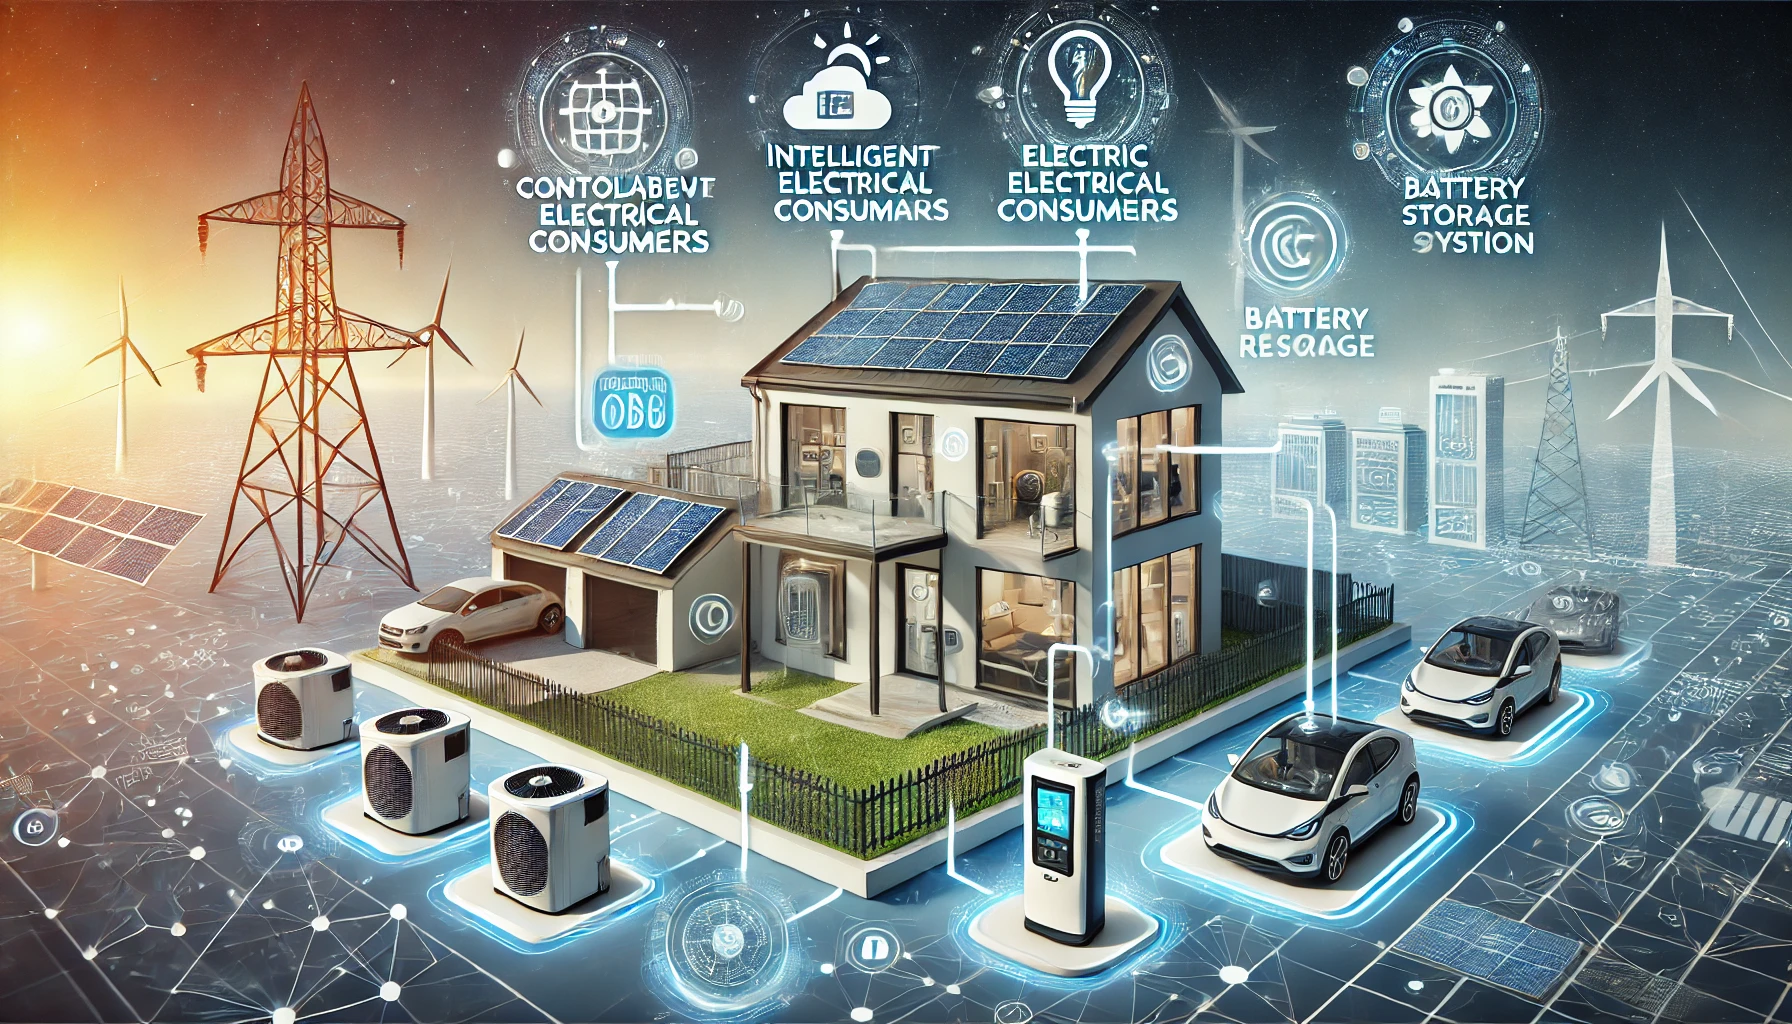
\includegraphics[width=1.05\paperwidth,viewport=0 -100 1600 1200]{images/Steuerbare_Verbraucher_2.png}%
}

\begin{frame}{Vielen Dank!}
   % Vereinslogo in der rechten oberen Ecke

   \begin{textblock*}{3cm}(0.8cm,2.2cm)  % Position (x,y) in cm anpassen
      
\includegraphics[width=3cm]{images/Logo_EWERH_eV_small.png}
   \end{textblock*}
   \vspace{2.5cm}
   \begin{center}
      \Huge Fragen?
   \end{center}
   \vfill
   \begin{minipage}{0.20\textwidth}
      \centering
      \begin{tikzpicture}
         \clip (0,0) circle (1cm);
         \node at (0,0) {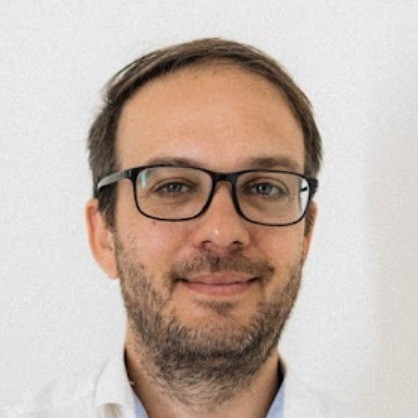
\includegraphics[width=2cm]{images/daniel_profil.jpeg}};
      \end{tikzpicture}
   \end{minipage}
   \hfill
   \begin{minipage}{0.75\textwidth}
      \begin{flushright}
         \footnotesize Daniel Glaser (Schatzmeister) \\
         \href{mailto:daniel.glaser@energiewende-erlangen.de}{daniel.glaser@energiewende-erlangen.de}
      \end{flushright}
   \end{minipage}%
\end{frame}

\usebackgroundtemplate{}